
\documentclass[a4paper,11pt]{article}
\usepackage[a4paper, margin=8em]{geometry}

% usa i pacchetti per la scrittura in italiano
\usepackage[french,italian]{babel}
\usepackage[T1]{fontenc}
\usepackage[utf8]{inputenc}
\frenchspacing 

% usa i pacchetti per la formattazione matematica
\usepackage{amsmath, amssymb, amsthm, amsfonts}

% usa altri pacchetti
\usepackage{gensymb}
\usepackage{hyperref}
\usepackage{standalone}

\usepackage{colortbl}

\usepackage{xstring}
\usepackage{karnaugh-map}

% imposta il titolo
\title{Appunti Calcolatori Elettronici}
\author{Luca Seggiani}
\date{2025}

% imposta lo stile
% usa helvetica
\usepackage[scaled]{helvet}
% usa palatino
\usepackage{palatino}
% usa un font monospazio guardabile
\usepackage{lmodern}

\renewcommand{\rmdefault}{ppl}
\renewcommand{\sfdefault}{phv}
\renewcommand{\ttdefault}{lmtt}

% circuiti
\usepackage{circuitikz}
\usetikzlibrary{babel}

% testo cerchiato
\newcommand*\circled[1]{\tikz[baseline=(char.base)]{
            \node[shape=circle,draw,inner sep=2pt] (char) {#1};}}

% disponi il titolo
\makeatletter
\renewcommand{\maketitle} {
	\begin{center} 
		\begin{minipage}[t]{.8\textwidth}
			\textsf{\huge\bfseries \@title} 
		\end{minipage}%
		\begin{minipage}[t]{.2\textwidth}
			\raggedleft \vspace{-1.65em}
			\textsf{\small \@author} \vfill
			\textsf{\small \@date}
		\end{minipage}
		\par
	\end{center}

	\thispagestyle{empty}
	\pagestyle{fancy}
}
\makeatother

% disponi teoremi
\usepackage{tcolorbox}
\newtcolorbox[auto counter, number within=section]{theorem}[2][]{%
	colback=blue!10, 
	colframe=blue!40!black, 
	sharp corners=northwest,
	fonttitle=\sffamily\bfseries, 
	title=Teorema~\thetcbcounter: #2, 
	#1
}

% disponi definizioni
\newtcolorbox[auto counter, number within=section]{definition}[2][]{%
	colback=red!10,
	colframe=red!40!black,
	sharp corners=northwest,
	fonttitle=\sffamily\bfseries,
	title=Definizione~\thetcbcounter: #2,
	#1
}

% disponi codice
\usepackage{listings}
\usepackage[table]{xcolor}

\definecolor{codegreen}{rgb}{0,0.6,0}
\definecolor{codegray}{rgb}{0.5,0.5,0.5}
\definecolor{codepurple}{rgb}{0.58,0,0.82}
\definecolor{backcolour}{rgb}{0.95,0.95,0.92}

\lstdefinestyle{codestyle}{
		backgroundcolor=\color{black!5}, 
		commentstyle=\color{codegreen},
		keywordstyle=\bfseries\color{magenta},
		numberstyle=\sffamily\tiny\color{black!60},
		stringstyle=\color{green!50!black},
		basicstyle=\ttfamily\footnotesize,
		breakatwhitespace=false,         
		breaklines=true,                 
		captionpos=b,                    
		keepspaces=true,                 
		numbers=left,                    
		numbersep=5pt,                  
		showspaces=false,                
		showstringspaces=false,
		showtabs=false,                  
		tabsize=2
}

\lstdefinestyle{shellstyle}{
		backgroundcolor=\color{black!5}, 
		basicstyle=\ttfamily\footnotesize\color{black}, 
		commentstyle=\color{black}, 
		keywordstyle=\color{black},
		numberstyle=\color{black!5},
		stringstyle=\color{black}, 
		showspaces=false,
		showstringspaces=false, 
		showtabs=false, 
		tabsize=2, 
		numbers=none, 
		breaklines=true
}


\lstdefinelanguage{assembler}{ 
  keywords={AAA, AAD, AAM, AAS, ADC, ADCB, ADCW, ADCL, ADD, ADDB, ADDW, ADDL, AND, ANDB, ANDW, ANDL,
        ARPL, BOUND, BSF, BSFL, BSFW, BSR, BSRL, BSRW, BSWAP, BT, BTC, BTCB, BTCW, BTCL, BTR, 
        BTRB, BTRW, BTRL, BTS, BTSB, BTSW, BTSL, CALL, CBW, CDQ, CLC, CLD, CLI, CLTS, CMC, CMP,
        CMPB, CMPW, CMPL, CMPS, CMPSB, CMPSD, CMPSW, CMPXCHG, CMPXCHGB, CMPXCHGW, CMPXCHGL,
        CMPXCHG8B, CPUID, CWDE, DAA, DAS, DEC, DECB, DECW, DECL, DIV, DIVB, DIVW, DIVL, ENTER,
        HLT, IDIV, IDIVB, IDIVW, IDIVL, IMUL, IMULB, IMULW, IMULL, IN, INB, INW, INL, INC, INCB,
        INCW, INCL, INS, INSB, INSD, INSW, INT, INT3, INTO, INVD, INVLPG, IRET, IRETD, JA, JAE,
        JB, JBE, JC, JCXZ, JE, JECXZ, JG, JGE, JL, JLE, JMP, JNA, JNAE, JNB, JNBE, JNC, JNE, JNG,
        JNGE, JNL, JNLE, JNO, JNP, JNS, JNZ, JO, JP, JPE, JPO, JS, JZ, LAHF, LAR, LCALL, LDS,
        LEA, LEAVE, LES, LFS, LGDT, LGS, LIDT, LMSW, LOCK, LODSB, LODSD, LODSW, LOOP, LOOPE,
        LOOPNE, LSL, LSS, LTR, MOV, MOVB, MOVW, MOVL, MOVSB, MOVSD, MOVSW, MOVSX, MOVSXB,
        MOVSXW, MOVSXL, MOVZX, MOVZXB, MOVZXW, MOVZXL, MUL, MULB, MULW, MULL, NEG, NEGB, NEGW,
        NEGL, NOP, NOT, NOTB, NOTW, NOTL, OR, ORB, ORW, ORL, OUT, OUTB, OUTW, OUTL, OUTSB, OUTSD,
        OUTSW, POP, POPL, POPW, POPB, POPA, POPAD, POPF, POPFD, PUSH, PUSHL, PUSHW, PUSHB, PUSHA, 
				PUSHAD, PUSHF, PUSHFD, RCL, RCLB, RCLW, MOVSL, MOVSB, MOVSW, STOSL, STOSB, STOSW, LODSB, LODSW,
				LODSL, INSB, INSW, INSL, OUTSB, OUTSL, OUTSW
        RCLL, RCR, RCRB, RCRW, RCRL, RDMSR, RDPMC, RDTSC, REP, REPE, REPNE, RET, ROL, ROLB, ROLW,
        ROLL, ROR, RORB, RORW, RORL, SAHF, SAL, SALB, SALW, SALL, SAR, SARB, SARW, SARL, SBB,
        SBBB, SBBW, SBBL, SCASB, SCASD, SCASW, SETA, SETAE, SETB, SETBE, SETC, SETE, SETG, SETGE,
        SETL, SETLE, SETNA, SETNAE, SETNB, SETNBE, SETNC, SETNE, SETNG, SETNGE, SETNL, SETNLE,
        SETNO, SETNP, SETNS, SETNZ, SETO, SETP, SETPE, SETPO, SETS, SETZ, SGDT, SHL, SHLB, SHLW,
        SHLL, SHLD, SHR, SHRB, SHRW, SHRL, SHRD, SIDT, SLDT, SMSW, STC, STD, STI, STOSB, STOSD,
        STOSW, STR, SUB, SUBB, SUBW, SUBL, TEST, TESTB, TESTW, TESTL, VERR, VERW, WAIT, WBINVD,
        XADD, XADDB, XADDW, XADDL, XCHG, XCHGB, XCHGW, XCHGL, XLAT, XLATB, XOR, XORB, XORW, XORL},
  keywordstyle=\color{blue}\bfseries,
  ndkeywordstyle=\color{darkgray}\bfseries,
  identifierstyle=\color{black},
  sensitive=false,
  comment=[l]{\#},
  morecomment=[s]{/*}{*/},
  commentstyle=\color{purple}\ttfamily,
  stringstyle=\color{red}\ttfamily,
  morestring=[b]',
  morestring=[b]"
}

\lstset{language=assembler, style=codestyle}

% disponi sezioni
\usepackage{titlesec}

\titleformat{\section}
	{\sffamily\Large\bfseries} 
	{\thesection}{1em}{} 
\titleformat{\subsection}
	{\sffamily\large\bfseries}   
	{\thesubsection}{1em}{} 
\titleformat{\subsubsection}
	{\sffamily\normalsize\bfseries} 
	{\thesubsubsection}{1em}{}

% tikz
\usepackage{tikz}

% float
\usepackage{float}

% grafici
\usepackage{pgfplots}
\pgfplotsset{width=10cm,compat=1.9}

% disponi alberi
\usepackage{forest}

\forestset{
	rectstyle/.style={
		for tree={rectangle,draw,font=\large\sffamily}
	},
	roundstyle/.style={
		for tree={circle,draw,font=\large}
	}
}

% disponi algoritmi
\usepackage{algorithm}
\usepackage{algorithmic}
\makeatletter
\renewcommand{\ALG@name}{Algoritmo}
\makeatother

% disponi numeri di pagina
\usepackage{fancyhdr}
\fancyhf{} 
\fancyfoot[L]{\sffamily{\thepage}}

\makeatletter
\fancyhead[L]{\raisebox{1ex}[0pt][0pt]{\sffamily{\@title \ \@date}}} 
\fancyhead[R]{\raisebox{1ex}[0pt][0pt]{\sffamily{\@author}}}
\makeatother

\begin{document}
% sezione (data)
\section{Lezione del 24-02-25}

% stili pagina
\thispagestyle{empty}
\pagestyle{fancy}

% testo
\subsection{Introduzione al corso}
Continuiamo lo studio di una particolare architettura per calcolatori, a partire da quanto detto riguardo alle reti logiche, introducendo i concetti di \textbf{interruzione}, \textbf{protezione} e \textbf{memoria virtuale}.
Questi 3 strumenti ci permetterano di realizzare il paradigma della \textbf{multiprogrammazione}, cioè di far eseguire ad una macchina con un singolo processore più programmi contemporaneamente.
Non si pensi questo significhi avere più processori, in quanto il corso riguarda esclusivamente processori \textit{single-threading}.

\subsection{Architettura}
L'archittettura di riferimento è quella classica, composta da \textbf{CPU}, \textbf{memoria} e \textbf{I/O} interconnessi da un \textbf{bus}:

\begin{center}
	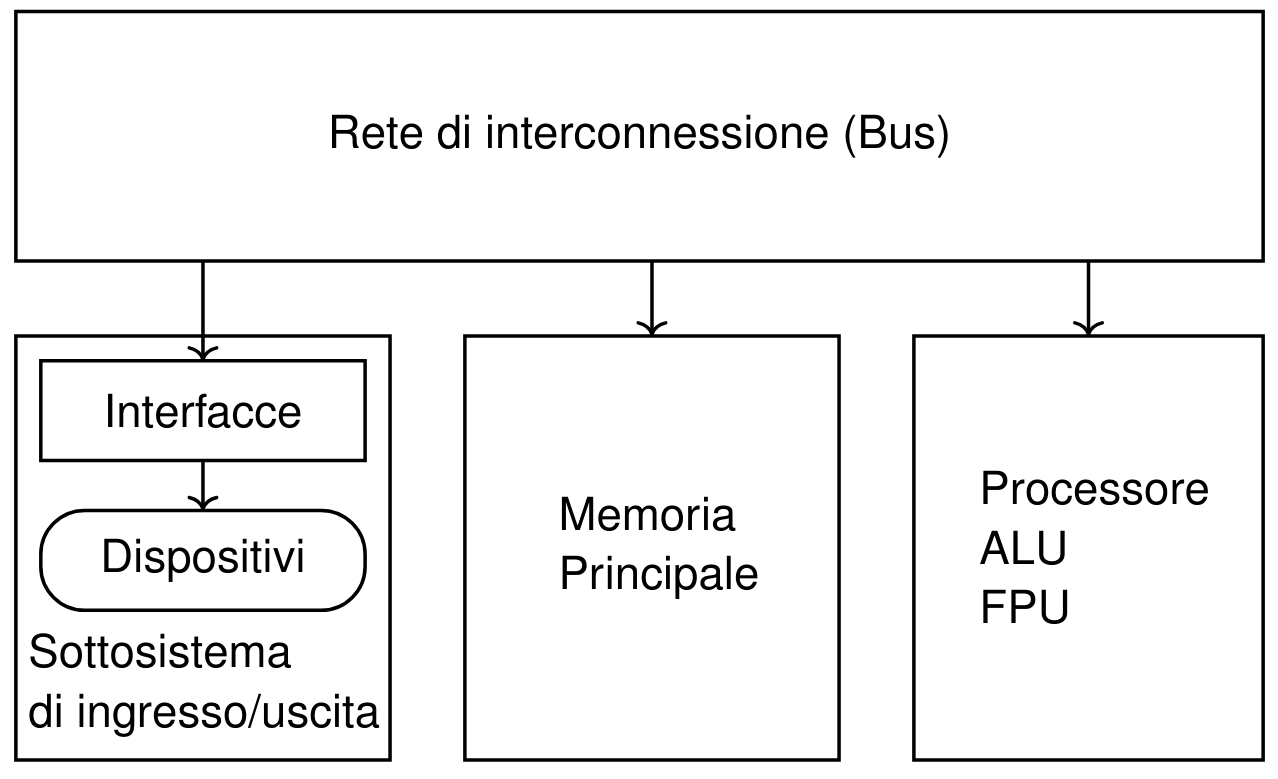
\includegraphics[scale=0.35]{../figures/struttura_calc.png}
\end{center}

Durante lo studio di un archiettura è oppurtuno porsi la domanda \textit{"chi fa cosa?"}, che fornisce determinati \textit{chi} ai determinati \textit{cosa} forniti da un opportuno livello di astrazione (transistor, porte logiche, diagrammi funzionali, ecc...).

La domanda che potremo porci adesso è \textit{"chi comanda?"} all'interno dell'architettura vista.
La risposta più giusta è quella del \textbf{software}: l'architettura è fatta per \textit{eseguire} software.

Per convincerci di questo possiamo sostituire la domanda \textit{"chi fa cosa?"} con la domanda \textit{"chi sa cosa?"}.

\begin{itemize}
	\item 
La \textbf{CPU} conosce lo stato corrente dei registri e l'istruzione in esecuzione.
Fra un'istruzione e l'altra non c'è alcun bisogno di sapere cosa è accaduto finora, e cosa accadrà in futuro, ma solamente l'istruzione corrente.
Quindi si può pensare che la CPU non \textit{sa} qual'è l'obiettivo della computazione, ma si limita a portarla avanti.

	\item
La \textbf{memoria} è un oggetto passivo, che contiene il programma, ma si limita a restiture i dati richiesti quando sono richiesti.
Notiamo che le memorie che usiamo sono ad \textbf{accesso casuale}, ergo nessuno scorre alla ricerca di indirizzi, ma si può leggere e scrivere in posizioni arbitrarie in tempo pressoché costante.
La memoria contiene \textbf{sempre} qualcosa, che questo sia significativo o meno, e la sua tipizzazione dipende solamente dalle intenzioni del programmatore.
	
	\item
L'\textbf{I/O} è il componente più variegato dell'architettura.
L'unica costante che rende la comunicazione con le periferiche più facile è la presenza di un interfaccia, che riduce tale comunicazione ad una semplice lettura o scrittura nello spazio di I/O.
La differenza fra le letture e scritture nello spazio di I/O e lo spazio di memoria è la possibile presenza di \textbf{effetti collaterali}, cioè effetti non riconducibili alla sola variazione di stato di una locazione di memoria.
Inoltre la CPU non è l'unica a scrivere nello spazio di I/O, in quanto questo può essere fatto anche dalle periferiche stesse.

	\item
Il \textbf{bus} è un insieme di linee (\textit{fili}), che trasportano ciò che ogni componente sta comunicando in un dato momento.
Ogni componente vede ciò che viene scritto sul bus in qualsiasi momento, e l'indirizzamento di locazioni specifiche nello spazio di memoria o nello spazio di I/O viene fatto attraverso \textbf{maschere} di indirizzo. 
\end{itemize}

\subsubsection{Flusso di controllo}
Abbiamo visto come la CPU si limita a prelevare ed eseguire istruzioni nel ciclo di \textbf{fetch-execute}.
L'istruzione successiva alla corrente, il cui indirizzo viene scritto nell'\textbf{instruction pointer}, viene decisa dall'istruzione corrente stessa (si pensi alle istruzioni di salto).
Il \textbf{flusso di controllo} è quindi deciso dall'istruzioni stesse, cioè dal programma.

Vedremo che mentre la struttura del calcolatore va a complicarsi, il flusso di controllo smette di essere completamente sequenziale (anche oltre alle istruzioni di salto), sopratutto grazie al meccanismo che introdurremo di \textit{interruzione}. 

\subsubsection{Bootstrap}
Il \textbf{bootstrap} è un processo secondo il quale si porta il sistema in un certo stato di esecuzione, apparentemente impossibile, o comunque molto difficile, da raggiungere.
Ad esempio, il compilatore del linguaggio C è scritto esso stesso in linguaggio C.
La domanda naturale è \textit{"come è stato compilato il compilatore?"}.
La risposta è un processo di boostrap, usando o un compilatore presesistente, magari che implementa un sottoinsieme parziale del C, o scrivendo l'intero compilatore in linguaggio macchina, cioè assemblando codice assembler.

Il boostrap si rende necessario anche all'avvio del calcolatore, per il caricamento del programma all'interno della memoria e l'inizio dell'esecuzione.
Nei calcolatori moderni questo viene fatto attraverso la \textbf{ROM}, cioè una memoria a sola lettura che contiene un programma di bootstrap.
All'avvio il processore è impostato in modo che al reset prenda come indirizzo proprio quello della ROM, e quindi inizi ad eseguire il programma di boostrap.
All'interno della ROM si trova, nei calcolatori moderni, il \textbf{BIOS} (o \textit{UEFI}, nei sistemi moderni), che ha il solo compito di impostare alcune periferiche di base e caricare il sistema operativo.

\par\medskip 

Iniziamo quindi ad approfondire, uno per uno, i moduli dell'architettura.

\subsection{Memoria}
La memoria è un insieme contiguo di locazioni di memoria, che nelle architetture moderne sono rappresentate da byte.
Storicamente, la memoria era indirizzata a \textit{parole}, cioè insiemi di bit coincidenti in dimensioni coi registri del processore.
Una parola poteva essere di più byte, mentre oggi le memorie sono accessibili ai singoli byte.
Ad esempio, le memorie usate nell'architettura Intel x86 sono accessibili ad 1 byte (\lstinline|MOVB|), 2 byte (\lstinline|MOVW|), 4 byte (\lstinline|MOVL|), e 8 byte (\lstinline|MOVQ|).

Il fatto che la memoria dell'architettura x86 sia organizzata a \textit{parole} da 8 byte (in particolare è cosi nella versione a 64 bit, x86\_64, che chiameremo semplicemente x86) comporta che cambi il modo stesso in cui vediamo la memoria.
Invece di vedere solo byte contigui, infatti, possiamo immaginare la memoria come organizzata in \textbf{righe}, a loro volta divise in 8 byte:

\begin{table}[h!]
	\center 
	\begin{tabular} { c || c | c | c | c | c | c | c | c || c }
		\bfseries Numero di riga & +7 & +6 & +5 & +4 & +3 & +2 & +1 & +0 & \bfseries Indirizzo di riga \\
		\hline
		0 & & & & & & & & & 0 \\
		\hline
		1 & & & & & & & & & 8 \\ 
		\hline
		2 & & & & & & & & & 16 \\ 
		\hline
		... & & & & & & & & & ...
	\end{tabular}
\end{table}

\subsubsection{Endianess}
Notiamo che la posizione in memoria del byte più significativo di una parola (in questo caso consideriamo una "parola" da 8 byte, da cui si ricavano tutte le altre misure) determina l'\textit{endianess} dell'architettura.
In particolare, se l'ultimo byte sta in fondo nella memoria, si dice \textbf{big-endian}, mentre se viceversa l'ultimo byte viene per primo nella memoria, si dice \textbf{little-endian}.

L'architettura Intel x86 che andiamo a considerare è little-endian, come lo sono la maggior parte delle architetture moderne.
Un esempio di utilizzo del big-endian e nella trasmissione di dati attraverso il protocollo IP, usato nelle comunicazioni Internet.

Il formalismo introdotto nel paragrafo precedente si dimostra utile anche da questo punto di vista: scrivendo le parole da destra verso sinistra, cioè a offset nella parola crescenti verso sinistra, si ha che il MSB finisce a sinistra, come suggerirebbe il senso di scrittura naturalsd.

\subsubsection{Allineamento}
Indicheremo con \textbf{offset} la distanza in byte fra due locazioni di memoria, intesa come il numero di locazioni che vanno saltate per raggiungere un indirizzo a partire dall'altro.
In questo ha senso parlare anche di offset \textit{negativi}.

Visto che lo spazio di memoria è effettivamente ciclico, cioè si ha \textit{wrap-around} ai suoi capi, si ha che gli offset rimangono validi \textbf{modulo} la dimensione dello spazio di memoria, che è sempre $2^n$, con $n$ nel nostro caso uguale a 64.

Il \textit{wrap-around} si comporta bene con gli offset, ma lo stesso non si può dire per quanto riguarda \textbf{intervalli} di byte.
Preso un certo intervallo $[x, y)$, quindi, si ha che questo contiene gli indirizzi $\{n \, | \, x \leq n < y\}$, ammesso che $x < y$, cosa che risulta falsa nel caso di intervalli che hanno \textit{wrap-around}. 
Decidiamo di non considerare intervalli di questo tipo.
Questo rende necessaria un'eccezione per intervalli che comprendono l'ultimo byte: in questo caso è concesso $[x, 0)$, con 0 che indica il fondo dello spazio di memoria.

Veniamo quindi all'\textbf{allineamento}.
Dire che un indirizzo è allineato ad un numero $n$ significa dire che quell'indirizzo è un multiplo di $n$.
Chiaramente, conviene scegliere $n$ potenze di 2.
In questo caso, per riconoscere se un indirizzo è allineato a $2^k$, basta guardare i suoi primi $k$ bit.

Si dice spesso che oggetti sono \textit{allineati alla parola}, ecc...
Questo significa che sono allineati alla \textit{dimensione} della parola specificata.
Altrimenti, si può dire che un oggetto è allineato \textit{naturalmente}, nel caso in cui sia allineato alla dimensione di stesso.

Infine, il \textbf{confine} di un oggetto è l'indirizzo che lo delimita dal resto dello spazio di memoria.

\end{document}
